\section*{Magnetometer Mapping}
    By knowing a box containing the magnetometer and its measuring range, we are able to find all the points seen for sure and all the points that could be seen by the magnetometer. This allows us to recover the coverage of the area by the magnetometer.

    \begin{figure}[!htb]
        \centering
        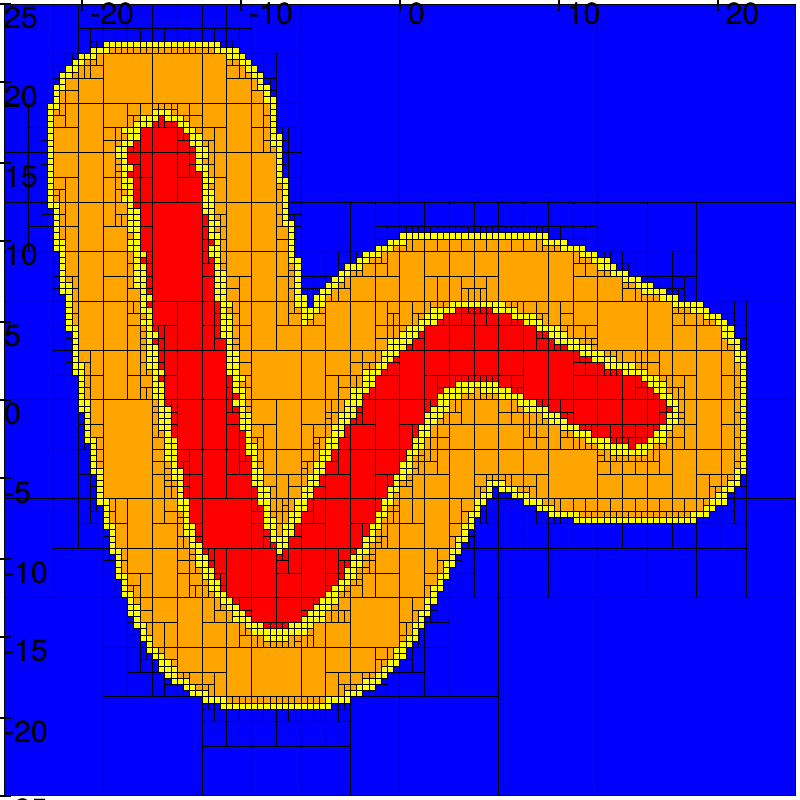
\includegraphics[width=0.4\textwidth]{imgs/thickset_fine.png}
        \caption{\label{fig:thickset} Coverage of the map by the magnetometer using Thicksets}
    \end{figure}

    The \textsc{Figure}~\ref{fig:thickset} shows us these two sets. The blue set is the unseen area, the orange set is the area maybe seen and the red set is the area seen for sure by the magnetometer. The yellow set forms the uncertain boundary between the other sets, which can be adjusted.